\documentclass[12pt]{article}
\usepackage[utf8]{inputenc}
\usepackage{amsmath}
\usepackage{hyperref}
\usepackage{graphicx}
\usepackage[swedish]{babel}
\title{Andragradsfunktioner}
\date{}
\begin{document}
  \maketitle
  
  
  
  \section{Introduktion}
  Det här dokumentet kommer från en fritt tillgänglig text på webbplatsen GitHub (se \url{https://github.com/Itangalo/Andragradsfunktioner}).
  Alla som är intresserade är inbjudna att föreslå och diskutera ändringar och förbättringar.
  Det kan man antingen göra genom att starta diskussioner i projektets ``issue queue'' (alternativt kommentera i befintliga diskussioner), eller genom att göra en kopia (``klon'') av hela projektet och redigera så mycket man vill.
  Om man är nöjd med sina ändringar, och vill att de ska tas in i ursprungliga dokumentet, kan man markera detta -- så kan förslaget diskuteras av andra inblandade.

  Innehållet i det här projektet är tillgänglig under Creative Commons-licens \href{http://creativecommons.org/licenses/by-nc-sa/3.0/}{attribution+non-commercial+share alike}.


  \section{Första skisser}
  
  (Det här är bara första skisser på upplägg av innehåll i dokumentet.)

  \subsection{Översikt av egenskaper för andragradsfunktioner.}
  Andragradsfunktioner har en högsta eller lägsta punkt, vilket gör dem användbara för att modellera vissa typer av samband.
  (Utgångspunkt i sådana samband!)
  Vad extrempunkt och extremvärde betyder, och varför de är viktiga begrepp i tillämpad matematik.

  \subsection{Hur uttrycket $f(x) = a(x+d)^2+e$ beter sig}
  Det finns olika sätt att representera andragradsuttryck, och $a(x+d)^2+e$ är en form som är praktisk för att se engenskaper hos funktioner.
  Utforskande av hur de olika parametrarna påverkar funktionens graf, framförallt hur $d$ och $e$ hänger samman med extrempunkt/extremvärde.
  (Bifogad GeoGebra-demonstration!)
  Fördjupning: Parametrarna $d$ och $e$, och translation av funktioner.
  
  \subsection{Andragradsekvationer}
  Motivering av ekvationer av typen $a(x+d)^2+e=k$.
  Hur man löser sådana ekvationer, med utgångspunkt i potensekvationen $x^2 = k$.
  Fördjupning: Jämförelse med substitutionen $t=x+d$.

  \subsection{Kvadratkomplettering med ansättning}
  Introduktion av andragradsuttryck på formen $ax^2+bx+c$, och hur parametern $c$ avspeglas i funktionens graf.
  Resonemang kring att det finns något uttryck $a(x+d)^2+e$ som representerar varje uttryck på formen $ax^2+bx+c$.
  Kvadreringsregler: utveckla uttryck på formen $(a+b)^2$ eller $(a-b)^2$.
  (Inklusive länk till digital mängdträning, som även omfattar andra parentesmultiplikationer.)
  Hur man kan översätta formen $ax^2+bx+c$ till kvadratkompletterad form (genom ansättning).
  Fördjupning: Vad ansättning egentligen innebär.
  
  \subsection{Överblivet}
  \begin{itemize}
    \item Faktorisering som genväg för att lösa andragradsekvationer
    \item Konjugatregeln. (Ha tillsammans med kvadreringsreglerna?)
    \item Komplexa tal och komplexa lösningar till andragradsekvationer
    \item Hur man kan hitta parametrarna $a$/$d$/$e$ eller $a$/$b$/$c$ från givna punkter
    \item Symmetrilinje för andragradsfunktioner
  \end{itemize}
  
  \begin{figure}
  \centering
  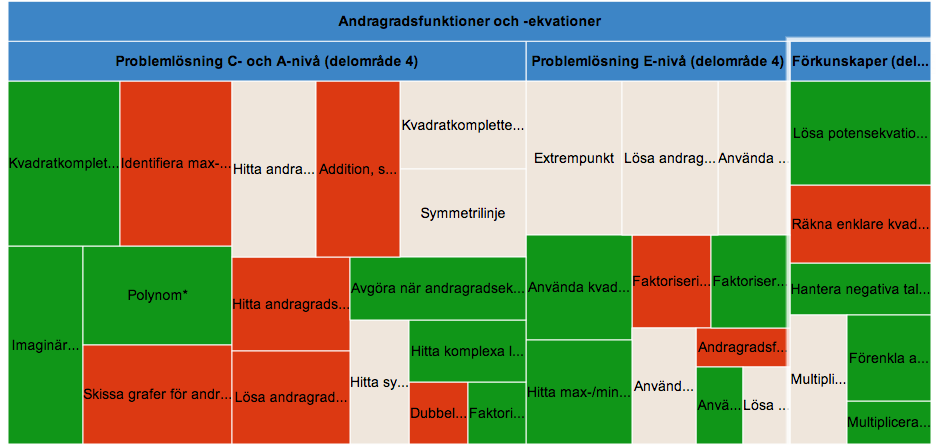
\includegraphics[width=0.3\textwidth]{bilder/testbild.png}
  \caption{\label{fig:testbild}Det här är bara ett test, för att se hur det fungerar att bädda in bilder.}
  \end{figure}

  \section{Varför andragradsfunktioner?}

Tidigare i kursen har vi tittat på linjära funktioner.
De är användbara i många olika sammanhang, inte minst för att skapa modeller för hur olika saker hänger samman:
hur fattigdom påverkar livslängd i ett land, hur koldioxidutsläpp påverkar globala medeltemperaturen, hur pluggtid påverkar hur man lyckas i skolan, med mera.

Men det finns också samband där det \emph{inte} är lyckat att använda räta linjer för att skapa modeller.
Här är ett exempel.

\begin{figure}
  \centering
  \includegraphics[width=0.3\textwidth]{bilder/bensinforbrukning.png}
  \caption{\label{fig:bensinförbrukning}Bensinförbrukning vid olika hastigheter (för en viss bilmodell).}
\end{figure}

Diagrammet visar hur bensinförbrukningen för en viss bilmodell påverkas av hur fort man kör.
Förbrukningen ökar eller minskar inte med någon jämn takt -- istället verkar den visa att det finns en lägsta bensinförbrukning om man kör ca 60--80 km/h.
Om vi försökte beskriva det här sambandet med en rät linje skulle vi helt missa att det finns en bästa hastighet att hålla, eftersom en rät linje skulle visa att bensinförbrukningen hela tiden ökar (eller minskar, beroende på lutning).

Här är ett annat exempel.

\begin{figure}
  \centering
  \includegraphics[width=0.3\textwidth]{bilder/biljettpriser.png}
  \caption{\label{fig:biljettpriser}Total vinst vid olika priser på bussbiljetter.}
\end{figure}

Det här diagrammet visar (ett påhittat) försök med olika biljettpriser på bussen, i en svensk stad.
Med höga priser gör bussbolaget mycket vinst per biljett, men samtidigt är det få personer som köper biljetter.
Med låga priser är det många som väljer att åka buss, men vinsten för varje biljett blir mindre.
Någonstans i mitten ligger det ``bästa'' biljettpriset (åtminstone om målet är att maximera vinsten).

\subsection {Andragradsfunktioner och extrempunkter}

För att modellera samband som har en högsta eller lägsta punkt använder man ofta något som heter \emph{andragradsfunktioner}.
Att de kallas andragradsfunktioner beror på att de innehåller en term med $x^2$ (medan räta linjer skulle kunna kallas förstagradsfunktioner, eftersom de bara innehåller $x^1$).

När vi studerade räta linjen tittade vi särskilt på saker som riktningskoefficient ($k$-värde) och skärning med y-axel ($m$-värde).
För andragradsfunktioner är det andra egenskaper som är intressanta, och den viktigaste av dem är \emph{extrempunkter} eller \emph{extremvärden}.

\begin{itemize}
  \item En \textbf{extrempunkt} är andragradsfunktionens vändpunkt -- det vill säga där funktionen har sitt högsta eller lägsta (mest extrema) värde. (Det är alltså en punkt med både x- och y-värde.)
  \item Ett \textbf{extremvärde} är funktionens värde i extrempunkten. (Det är alltså ett tal.)
  \item Ett \textbf{maximumvärde} är ett extremvärde som är det högsta möjliga, och alltså ligger på en kurva som går upp och sedan ner.
  \item Ett \textbf{minimumvärde} är ett extremvärde som är det lägsta möjliga, och alltså ligger på en kurva som går ned och sedan upp.
  \item En \textbf{parabel} är en graf för en andragradsfunktion.
\end{itemize}

En av de viktigaste användningsområdena för matematik är att hitta extrempunkter för olika samband, vilket inte är så konstigt.
Med hjälp av matematiska analyser kan man få väl underbyggda svar på frågor som:
Hur mycket av kommunbudgeten bör läggas på snöröjning?
Hur mycket ska man träna på gymmet för att få bästa möjliga effekt?
Hur ska vattenreningsverk styras för att dra så lite energi som möjligt?

I många situationer är samband och extrempunkter svåra att hitta, och kräver stora studier.
I det här avsnittet i kursen ska vi titta på några enklare exempel, och se hur vi kan använda andragradsfunktioner för att hitta extrempunkter.


  
  \section{Att tolka andragradsuttryck}

Ekvationer för räta linjer kan skrivas på en rad olika sätt -- ekvationerna $y = -2x + 3$, $y + 2x = 3$ och $y + 2x - 3 = 0$ beskriver alla samma linje.
Beroende på hur man skriver ekvationen går det lättare eller svårare att läsa av olika egenskaper för linjen, som lutning eller skärning med y-axeln.

Precis som räta linjer, kan andragradsfunktioner skrivas på ett antal olika sätt.
Det sätt man vanligtvis ser är \mbox{$f(x) = ax^2 + bx + c$}, exempelvis $y=2x^2 - 12x + 19$, men vi kommer till en början att fokusera på formen \mbox{$f(x) = a(x+d)^2+e$} istället -- exempelvis $y=2(x-3)^2+1$.

Det sättet att skriva andragradsuttryck på kallas \emph{kvadratkompletterad form} (eftersom uttrycket består av en kvadrat som kompletterats med en konstant).
Om en andragradsfunktion är skriven på kvadratkompletterad form är det lätt att hitta extrempunkter och extremvärden för funktionen, och det går också relativt lätt att lösa ekvationer som består av kvadratkompletterade andragradsuttryck.

\subsection{Hitta extremvärdet för en andragradsfunktion}

\begin{figure}
  \centering
  \includegraphics[width=0.3\textwidth]{bilder/2(x-3)^2+1.png}
  \caption{\label{fig:2(x-3)^2+1}Grafen till funktionen $f(x)=2(x-3)^2+1$.}
\end{figure}

Ta en titt på grafen till funktionen $f(x) = 2(x-3)^2+1$.
Vi kan se från funktionens graf att det minsta värdet funktionen kan anta är 1, och vi kan se att det värdet får funktionen när $x=3$.
Men vi kan läsa samma information direkt ur funktionsuttrycket också. Hur då?

Funktionsuttrycket består av två delar -- en kvadrat $2(x-3)^2$ vars värde bestäms av $x$, och en konstant 1.
Beroende på vilket värde vi ger $x$ kommer kvadratdelen att bli olika stor, men den kommer alltid att bli \emph{positiv} (eftersom även negativa värden blir positiva när de kvadreras).
Vi skulle alltså kunna tolka funktionen som att vi har talet 1, och ska lägga till ett annat tal som är 0 eller större beorende på vad x är.

Ser man funktionsuttrycket på det viset är det ganska lätt att se att 1 är det minsta värdet som funktionen kan ha.
Vi kan i allmänhet dra slutsatsen att om en andragradsfunktion beskrivs av $f(x)=a(x+d)^2+e$ är funktionens extremvärde $e$.

Om vi inte bara är intresserade av extrevärdet, utan även \emph{extrempunkten}, räcker det inte att hitta y-värdet för extrempunkten -- vi måste också hitta vilket x-värde som ger funktionen dess extremvärde.
När blir $f(x) = 2(x-3)^2+1$ så litet som möjligt?
Ja, om funktionen består av talet 1 plus en kvadratterm, måste funktion få sitt lägsta värde när kvadraten är noll.
När blir $2(x-3)^2 = 0$? Jo, när värdet inomparentes blir noll -- det vill säga när $x = 3$.
Vi kan i allmänhet dra slutsatsen att om en andragradsfunktion beskrivs av $f(x)=a(x+d)^2+e$ är x-koordinaten för funktionens extrempunkt $-d$.

\subsubsection{Positiva och negativa andragradsfunktioner}

\begin{figure}
  \centering
  \includegraphics[width=0.3\textwidth]{bilder/-3(x+1)^2+4.png}
  \caption{\label{fig:-3(x+1)^2+4}Grafen till funktionen $f(x)=-3(x+1)^2+4$.}
\end{figure}

I den här grafen syns en annan andragradsfunktion, nämligen $f(x)=-3(x+1)^2+4$.
Vi kan, både från grafen och funktionsuttrycket, se att funktionens extrempunkt är $(-1, 4)$.
Men extrempunkten är en \emph{maximumpunkt} -- den högsta punkten på kurvan -- istället för en minimumpunkt.

Även detta kan vi läsa direkt från funktionsuttrycket:
Kvadrattermen är i det här fallet \emph{negativ}; i förra exemplet hade vi ``1 plus en kvadrat'', men här har vi istället ``4 \emph{minus} en kvadrat''.
Funktionens värde kommer alltså att vara \emph{som mest} 4, och det värdet får funktionen då kvadraten blir noll (det vill säga $x=-1$).

Vi kan i allmänhet dra slutsatsen att om faktorn $a$ är positiv har funktionen en minimumpunkt, och om $a$ är negativ har funktionen en maximumpunkt.
Man brukar ibland prata om positiva och negativa andragradsfunktioner, vilket betyder att $a$-värdet är positivt eller negativt.

\subsection{Symmetrilinje}



\subsubsection{Termer och uttryck}

\begin{itemize}
  \item Andragradsuttryck på allmän form: $ax^2+bx+c$
  \item Andragradsuttryck på kvadratkompletterad form: $a(x+d)^2+e$
  \item En andragradsfunktion $f(x)=a(x+d)^2+e$ har extremvärdet $e$.
  \item En andragradsfunktion $f(x)=a(x+d)^2+e$ har extrempunkten $(-d, e)$.
  \item $a > 0$ betyder att funktionen har en minimumpunkt (och är en positiv andragradsfunktion).
  \item $a < 0$ betyder att funktionen har en maximumpunkt (och är en negativ andragradsfunktion).
\end{itemize}

\subsection{Uppgifter och övningar}

\url{http://www.geogebratube.org/student/m115801}


\end{document}
